

Jako \orig{70} singulární budeme označovat takové vyrovnávací úlohy,
které vedou na singulární matici soustavy normálních rovnic a nejsou
proto klasickým postupem řešitelné. Snadno lze ověřit, že např. při
vyrovnání zprostředkujících resp. podmínkových pozorování bude úloha
singulární tehdy, je-li hodnost matice soustavy rovnic oprav
resp. podmínkových rovnic menší než počet jejich sloupců
resp. řádků. Singularita matice soustavy normálních rovnic signalizuje
sice obvykle určité nesrovnalosti ve formulaci vyrovnávací úlohy,
nelze z ní však ještě obecně soudit na neřešitelnost vyrovnávací
úlohy. Vedle singulárních úloh neřešitelných (např. odporující si
podmínkové rovnice) existují totiž úlohy řešitelné jednoznačně
(např. nadbytečné podmínkové rovnice), příp. i úlohy s větším počtem
řešení (např. nadměrný počet neznámých při vyrovnání zprostředkujících
pozorování).  Singulární úlohy nejsou přitom záležitostí jen
teoretickou - setkáváme se s nimi i ve výpočetní praxi. Je proto
oprávněné požadovat na univerzálním vyrovnávacím algoritmu, aby měl
následující vlastnosti

\begin{itemize}

\item[--] signalizoval singularitu úlohy

\item[--] nalezl řešení úlohy, pokud je jednoznačné

\item[--] nalezl alespoň jedno řešení úloh s větším počtem řešení

\item[--] umožnil identifikovat neřešitelné úlohy a příp. řešil místo
  nich modifikované, v některém smyslu blízké, regulární
  úlohy náhradní.
\end{itemize}

\noindent V dalším naznačíme jeden z možných způsobů zpracování singularit u
všech čtyř kategorií vyrovnávacích úloh. Nejprve uvedeme několik
obecných úvah.

Při vyrovnání zprostředkujících pozorování nechť je $A (m \times n)$
matice soustavy rovnic oprav, jejíž hodnost $h$ je menší než $n$.
Nechť
%
\begin{align*}
  \tag{8.1}
  h = n - k, \qquad k > 0.
\end{align*}
%
\noindent\orig{71}
%
Potom $h$ sloupců matice $A$ je lineárně nezávislých. Ostatní $k$
sloupce mohou být vyjádřeny jako jejich určité lineární
kombinace. Předpokládejme bez újmy na obecnosti, že první $h$
sloupce matice $A$, psané ve tvaru
%
\begin{align*}
  \tag{8.2}
  A = \vcenter{\hbox{
      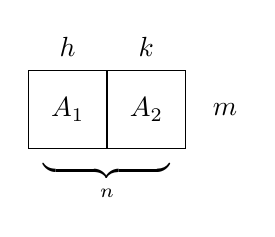
\begin{tikzpicture}{x=1cm,y=1cm}
        \draw(0.5,2.3) node{$h$};    \draw(1.5,2.3) node{$k$};
        \draw (0,1) rectangle (1,2); \draw(0.5,1.5) node{$A_1$};
        \draw (1,1) rectangle (2,2); \draw(1.5,1.5) node{$A_2$};
        \draw(2.5,1.5) node{$m$};
        \draw(1,.6) node{$\underbrace{\hskip 1.6cm}_n$};
      \end{tikzpicture}
  }}
\end{align*}
%
\noindent jsou lineárně nezávislé. Pak lze najít matici $\alpha$ $(h
\times k)$ takovou, že platí
%
\begin{align*}
  \tag{8.3} A_2 = A_1 \alpha ,
\end{align*}
%
kde i-tý (i=1,2,...,k) sloupec matice a obsahuje koeficienty,
vyjadřující i-tý sloupec matice $A_2$ jako lineární kombinaci sloupců
matice $A_1$. Máme-li nyní řešit vyrovnávací úlohu s maticí $A$
%
\begin{align*}
  \tag{8.4}     v = Ax + \ell,
\end{align*}
%
pak vzhledem k (8.2) a (8.3) můžeme psát
%
\begin{align*}
  \tag{8.5}
  v = \left[ A_1 A_2 \right] \left[
  \begin{array}{c}
    x_1  \\ x_2
  \end{array}
  \right]
  +
  \ell
  = A_1x' + \ell,
\end{align*}
%
kde jsme položili
\begin{align*}
  \tag{8.6}
  x' = x_1 + \alpha x_2 .
\end{align*}
%
Rovnice oprav
\begin{align*}
  \tag{8.7}
  v = A_1x' + \ell
\end{align*}
%
můžeme jednoznačně řešit metodou nejmenších čtverců, protože sloupce
matice $A_1$ $(m \times h)$ jsou podle předpokladu lineárně
nezávislé. Neznámé $x'$ nalezené řešením (8.7) jsou s hledanými
vektory neznámých $x_1$ a $x_2$ spojeny prostřednictvím rovnice (8.6).
Je zřejmé, že každá dvojice vextorů $x_1$ a $x_2$, vyhovující rovnici
(8.6) je řešením výchozí vyrovnávací úlohy (8.4). Docházíme tedy k
závěru, že při řešení popisované úlohy \Xemph{můžeme postupovat např. tak, že
$k$ neznámých $x_2$ volíme zcela libovolně a odpovídající hodnoty
$x_1$ najdeme ze vzorce (8.6) pomocí matice $\alpha$ jako rozdíl}
 \orig{72}
%
  \begin{align*}
    \tag{8.8}
    x_1 = x' - \alpha x_2 .
  \end{align*}

\noindent Klademe-li jednoduše $x_2=0$, pak znalost matice $\alpha$
není nutná, protože je přímo $x_1=x'$. Jinými slovy: v matici soustavy
rovnic oprav můžeme v takovém případě ignorovat všechny sloupce
submatice A. Někteří autoři [13] , [51] užívají jiného přístupu k
řešení úloh s lineárně závislými sloupci v matici $A$. Hledají
tzv. zobecněné normální řešení soustavy [13,str.76] , které opět vede
k minimálnímu součtu čtverců oprav a navíc splňuje podmínku
minimální délky
%
\begin{align*}
  \tag{8.9}
  \Vert x \Vert = \min.
\end{align*}


Při vyrovnání podmínkových pozorování signalizuje nalezení
lineárně závislého řádku v~matici soustavy podmínkových rovnic
jednu ze dvou situací


\begin{itemize}
\item[--] byla nalezena podmínková rovnice, která je důsledkem
  (lineární kombinací) ostatních rovnic,

\item[--] byla nalezena rovnice, která odporuje ostatním rovnicím.
\end{itemize}

\noindent V prvním přínadě zůstává jednoznačnost řešení úlohy metodou
nejmenších čtverců zachována, přestože matice soustavy normálních
rovnic je singulární. Ve druhém případě je úloha podle
\name{KRONECKEROVY} věty [37, str.78] neřešitelná -- hodnost matice
soustavy podmínkových rovnic $A^T$ (3.21) je totiž menší než hodnost
matice rozšířené $\left[A^Tu^T\right]$.


Singularita, kterou jsme se právě zabývali v souvislosti s
vyrovnáním zprostředkujících a podmínkových pozorování, se může
vyskytnout i u zbývajících dvou kategorif vyrovnávacích úloh.
Při vyrovnání zprostředkujících pozorování s podmínkami (IC)
může být hodnost matice
$\left[
  \begin{array}{c}
    A \\ B
  \end{array}
  \right]$
-- viz (5.1) a (5.2) -- menší než počet
neznámých a je pak stejně jako u vyrovnání zprostředkujících
pozorování např. možno hodnoty některých neznámých libovolně volit.
U~vyrovnání podmínkových pozorování s neznámými (CU) může být
podobně hodnost matice $\left[ A^T B^T\right]$  v (5.3) menší než počet
podmínkových rovnic a úloha nemusí mít řešení.

Úlohy \orig{73} typu IC a CU mohou být singulární ještě z další
příčiny. Jak je patrno ze (5.15) a (5.16) bude matice soustavy
normálních rovnic při řešení úloh typu IC singulární také
tehdy, nebudou-li všechny řádky matice $B$ v (5.2) lineárně
nezávislé, tj. bude-li hodnost matice $B$ menší než $m_2$. V závislosti na
hodnosti matice rozšířené $\left[B \ell_2\right]$ mohou pak být soustava (5.2)
a tedy i celá vyrovnávací úloha neřešitelné. Podobně lze dokázat,
že lineární závislost sloupců matice $B^T$ v (5.3) je příčinou
singularity matice soustavy normálních rovnic úloh typu CU. Ukazuje
se, že v takových případech nelze určit neznámé ze soustavy
podmínkových rovnic (5.3) jednoznačně. Stejně jako tomu bylo při
vyrovnání zprostředkujících oozorování, je např. možno některé
hodnoty neznámých libovolně volit, resp. některé neznámé vypustit.

Pro rozlišení budeme naposled popsanou singularitu označovat
jako singularitu druhého druhu, na rozdíl od singularity
prvního druhu, kterou jsme definovali předtím v souvíslosti nejprve
s vyrovnáním zprostředkujících a podmínkových pozorování.
Vyšetřeme nyní projevy singularit obou uvedených druhů při řešení
základních vyrovnávacích úloh ortogonalizačním algoritmem ORTON,
Současně popíšeme způsob zpracování singulárních úloh, kterého
užívá procedura ORTON3 (kap. 12).



\section{Zprostředkující pozorování}

Vyrovnání zprostředkujících pozorování algoritmem ORTON se
redukuje, jak jsme viděli v~kap.~6, na zobecněnou
ortogonalizaci např. ve tvaru (3.17).
%
\Xemph{ Singularita prvního druhu se potom podle našeho konstatování v
  kap. 2 projeví při ortogonalizaci základní submatice $A$ nulovou
  délku některého vektoru $\widetilde w_i$.}
%
Ortogonalizační algoritmus může na takovou situaci reagovat např.
tak, že upustí od normalizace vektoru $\widetilde w_i$, vynuluje všechny
prvky i-tého sloupce matice $W_0$ (3.18), tedy i prvky odpovídající
všem vedlejším submaticím matice $A_0$ (3.17) a přejde ke
zpracování dalších sloupců matice $A_0$. Při tomto postupu bude
ignorován sloupec $a_i$ matice soustavy rovnic oprav, hodnota neznámé $x_i$
%
bude \orig{74} rovna nule a bude pokládána za konstantu. Váhové
koeficlenty počítané podle (3.11), (3.13) a (3.14) jsou totiž také
nulové. Nulované prvky i-tého sloupce, zejména prvky $r_k$ $(k=1,
2,\ldots,i)$ odpovídající submatici $R^{-1}$ (3.18), je vhodné tisknout
Lze např. dokázat, že pomocí prvků $r_k$ mohou být jednoduše
vyjádřeny koeficienty v~rozkladu
%
\begin{align*}
  \tag{8.10}
  a_i = \sum_{j=1}^{i-1} (-r_j/r_i) a_j,
\end{align*}
%
vyjadřujícím i-tý sloupec matice $A$ jako lineární kombinaci
sloupců předcházejících.
%
\footnote{
Při užití zobecněné ortogonalizace ve formě popsané v kap. 2
je $r_i=1$. Vzorec (8.10) respektuje modifikaci algoritmu užitou
v proceduře ORTON) (kap. 12), kde dochází k jisté vstupní
normalizaci sloupců matice $A_0$ podle (12.4), V důsledku této úpravy
je obecně $r \ne 1$.
}
\footnote{
Pokud bylo užito tzv. selektivní varianty algoritmu (kap. 9),
Je obecně třeba počítat součet (3.10) pro $j=1,2,\ldots,n$.
}



\section{Podmínková pozorování}

\Xemph{Singularita prvního druhu se při vyrovnání podmínkových
  pozorování projeví analogicky jako v odst. 8.1 nulovou délkou
  některého vektoru $\widetilde w_i$}
%
při zobecněné ortogonalizaci
např. (3.34) $\rightarrow$ (3.35). Rovněž reakce algoritmu může být v
takovém případě stejná jako u vyrovnání zprostředkujících pozorování:
vynecháním normalizace vektoru $\widetilde w_i$, nulováním všech
prvků i-tého sloupce matice $W_0$ (3.35) a přechodem ke zpracování
dalších sloupců budou ignorovány ty podmínkové rovnice, které jsou
buď důsledkem jiných nebo jim odporují.


U vyrovnání podmínkových pozorování je třeba navíc najít kritérium pro
posouzení řešitelnosti podmínkových rovnic. Při jeho hledání můžeme
vyjít např. z následující úvahy. V kap. 3 jsme viděli, že výchozí
soustavě oodmínkových rovnic (3.21) odpovídá ekvivalentní soustava
(3.36) s maticí $W^T$ a absolutními členy $(u R^{-1})^T = -k^{*}$.
Nechť je nyní např. i-tý řádek matice $W^T$ nulový.  Je zřejmé, že
\Xemph{ekvivalentní soustava (3.36) a tedy i výchozí soustava (3.21)
  budou řešitelné právě tehdy, bude-li i odpovídající absolutní člen
  $-k_i^{*}$ roven nule}.
%
Vektor $-k^*$ ovšem známe -- je
%
\orig{75} určován ortogonalizačním algoritmem v posledním řádku matice
$W_0$ (3.35). V~případě lineárně závislého sloupce je
odpovídající složka $-k_i^*$ nulována;
v~proceduře je proto třeba pamatovat
na její včasný tisk. Potvrzuje se tak účelnost tisku prvků
odpovídajících vedlejším submaticím, zmíněná již při vyrovnání
zprostředkujících pozorování. Pokud bychom analogicky jako v
odst. 8.1 ortogonalizovali i jednotkovou submatici v levé
dolní části matice $A_0$ (3.34), můžeme podle (8.10) s využitím
tištěných hodnot najít i koeficienty, vyjadřující i-tý řádek
matice soustavy podmínkových rovnic jako lineární kombinaci
předcházejících řádků.



\section{Podmínková pozorování s neznámými}

Úlohy typu CU stejně jako IC mohou, jak jsme již uvedli,
vykazovat singularity dvojího druhu. Singularita prvního druhu se
při jejich řešení algoritmem ORTON projevuje ve čtvrtém kroku
algoritmu a to formou, s níž jsme se setkali již v odst. 8.2
resp. 8.1. Analogickými zásadami jako tam lze po zjištění
singularity řídit i další zpracování a analýzu takových úloh.

Studujme nyní projevy singularity druhého druhu úloh typu
CU, vyvolané lineární závislostí sloupců matice
%
\begin{align*}
  \tag{8.11}
  \left[
    \begin{array}{c}
      B_1^T \\ B_2^T
    \end{array}
    \right]
    \quad
    (n_1 \times m_2)
\end{align*}
%
v (7.18), při ortogonalizaci např. podle (7.20). Jsou-li sloupce
matice (8.11) lineárně závislé, pak čtvercová matice $B_1$ $(m_2
\times m_2)$ je singulární a navíc nelze najít ani žádnou permutaci
$m_2$ lineárně nezávislých sloupců matice $[ B_1 B_2 ]$.%
%
\footnote{ Vytváření vhodných permutací sloupců ortogonalizované
	matice se realizuje pomocí tzv. selektivní varianty
	ortogonalizačního algoritmu (kap. 9).}%
%
~V~každém případě bude tedy nejméně jeden sloupec matice $B_1$
lineární kombinací jejích ostatních sloupců a je zřejmé, že již v
prvním kroku algoritmu nastane situace, \Xemph{kdy délka některéno
  vektoru $\widetilde w_i$} (odpovídá základní submatici $B_1$)
\Xemph{bude nulová}. Singularity obou druhů se tedy projevují
analogickým způsobem; jediný rozdíl spočívá v tom,
%
\orig{76} že \Xemph{singularita prvního druhu se projevuje ve čtvrtém
  kroku algoritmu, zatímco singularita druhého druhu se projevuje již
  v jeho prvním kroku}.


V úvodu k této kapitole jsme naznačili, že jedna cesta řešení úloh
typu CU se singularitou druhého druhu může vést přes vypuštění
některých sloupců v matici (8.11) a tedy vypuštění řádků v
ortogonalizované matici $A$ (7.20), Ukazuje se, že zatímco vypouštění
sloupců ortogonalizované matice nečiní potíže, jak jsme ostatně viděli
v odst. 8.1 a 8.2, je vypouštění řádků spojeno se značnými
komplikacemi. Zdá se proto vhodnější volit odlišný
postup. Nejednoznačnost v určení neznámých nemusíme totiž odstraňovat
jenom volbou pevných hodnot nebo ignorováním některých z nich, ale
také tak, že počet neznámých ponecháme beze změny a připojíme nové
podmínky, jimž by neznámé měly vyhovovat. Je-li
%
\begin{align*}
  \tag{8.12}
  h = m_2 - k,  \quad k > 0
\end{align*}
%
hodnost matice (8.11), pak stačí připojit k podmínek, např. ve
tvaru
%
\begin{align*}
  \tag{8.13}
  B_3^T x = 0,
\end{align*}
%
kde matici $B_3^T$ $(k \times m)$ je ovšem třeba stanovit tak, aby hodnost
matice
%
\begin{align*}
  \tag{8.14}
  \left[
    \begin{array}{c}
      B_1^T \\ B_2^T \\ B_3^T
    \end{array}
    \right]
\end{align*}
%
byla rovna $m_2$ (požadavek lineární nezávislosti sloupců
doplněné matice). Řešení založené na připojení podmínek (8.13) je
zdánlivě složitější než vypouštění sloupců v (8.11). Jeho
realizace je však ve spojení s ortogonalizačním procesem velmi
jednoduchá. Stačí totiž pomocí vhodného generátoru náhodných
čísel postupně doplňovat zpracovávanou matici $A$ (7.20) sloupci
o struktuře
%
\orig{77}
%
\begin{align*}
  \tag{8.15}
  \vcenter{\hbox{
  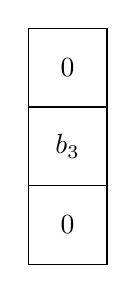
\begin{tikzpicture}[x=1cm,y=1cm]
    \draw (0,2) rectangle (1,3); \draw (0.5,2.5) node{$0$};
    \draw (0,1) rectangle (1,2); \draw (0.5,1.5) node{$b_3$};
    \draw (0,0) rectangle (1,1); \draw (0.5,0.5) node{$0$};
  \end{tikzpicture}}}
  \Punc{,}
\end{align*}
%
kde $b_3$ představuje sloupec matice $B_3$. Pokud by se ukázalo, že
některý generovaný vektor $b_3$, vede k příliš malé nebo dokonce
nulové hodnotě normy $\Vert\widetilde w_i\Vert$, stačí jej jednoduše nahradit
jiným.


Procedura ORTON3 generuje vedle sloupce (8.15) i nový řádek
matice $A$ (7.20). Generovaný řádek je tvořen nulami s výjimkou
pozice odpovídající generovanému sloupci, kam se ukládá
koeficient rovný jedné. Matici $A$, doplněnou generovaným sloupcem a
řádkem, lze potom znázornit schematem
%
\begin{align*}
  \tag{8.16}
  \vcenter{\hbox{
  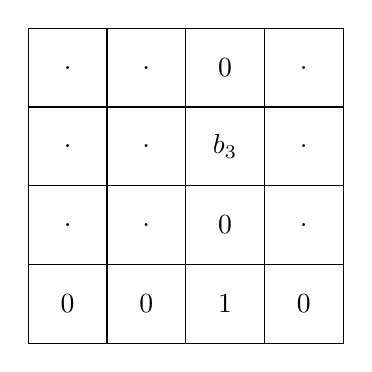
\begin{tikzpicture}[x=1cm,y=1cm]
    \draw (0,3) rectangle (1,4); \draw (0.5,3.5) node{$.$};
    \draw (0,2) rectangle (1,3); \draw (0.5,2.5) node{$.$};
    \draw (0,1) rectangle (1,2); \draw (0.5,1.5) node{$.$};
    \draw (0,0) rectangle (1,1); \draw (0.5,0.5) node{$0$};
    %
    \draw (1,3) rectangle (2,4); \draw (1.5,3.5) node{$.$};
    \draw (1,2) rectangle (2,3); \draw (1.5,2.5) node{$.$};
    \draw (1,1) rectangle (2,2); \draw (1.5,1.5) node{$.$};
    \draw (1,0) rectangle (2,1); \draw (1.5,0.5) node{$0$};
    %
    \draw (2,3) rectangle (3,4); \draw (2.5,3.5) node{$0$};
    \draw (2,2) rectangle (3,3); \draw (2.5,2.5) node{$b_3$};
    \draw (2,1) rectangle (3,2); \draw (2.5,1.5) node{$0$};
    \draw (2,0) rectangle (3,1); \draw (2.5,0.5) node{$1$};
    %
    \draw (3,3) rectangle (4,4); \draw (3.5,3.5) node{$.$};
    \draw (3,2) rectangle (4,3); \draw (3.5,2.5) node{$.$};
    \draw (3,1) rectangle (4,2); \draw (3.5,1.5) node{$.$};
    \draw (3,0) rectangle (4,1); \draw (3.5,0.5) node{$0$};
    %
  \end{tikzpicture}}}
  \Punc{,}
\end{align*}
%
kde submatice označené tečkou představují submatice v matici $A$
(7.20). Připojením řádku  je pamatováno na případy, kdy
součástí ortogonalizované matice je jednotková submatice, jak tomu
bylo např. v (7.8). Generovaný řádek v podstatě přizpůsobuje
tuto submatici rozměrům úlohy, které se změnily připojením
generovaného sloupce.

Ne závěr poznamenejme, že \Xemph{připojení podmínek} (8.13)
\Xemph{nemá vliv na výpočet oprav}, které se v případě singularity
druhého druhu určují jednoznačně.



\section{Zprostředkující pozorování s podmínkami}

Vyšetříme singularitu druhého druhu v úlohách typu IC, popsaných
definičními rovnicemi (7.5). O rovnicích (7.5) budeme předpokládat,
\orig{78} že nevykazují singularitu prvního druhu. Řešení úloh nechť
bylo hledáno ortogonalizací např. podle schematu (7.8).


V úlohách typu IC dochází k singularitě druhého druhu tehdy,
Je-li mezi podmínkovými rovnicemi v (7.5)
%
\begin{align*}
  \tag{8.17}
  0 = \left[
    \begin{array}{cc}
      B_1 & B_2
    \end{array}
    \right] x + \ell_2
\end{align*}
%
alespon jedna rovnice, která bud vyplývá z ostatních rovnice
nebo jim odporuje. Matice soustavy (8.17) má v takovém případě
analogické vlastnosti jako stejně značená matice v odst. 8.3. Platí
proto i stejný závěr, podle něhož se \Xemph{singularita druhého druhů
  projevuje v prvním kroku algoritmu ORTON nulovou délkou
  některého vektoru $\widetilde w_i$}.

V odst. 8.2 jsme při zjištění lineární závislosti řádků matice
soustavy podmínkových rovnic přikročili k eliminaci (vyloučení) vhodně
vybraných podmínkových rovnic. Užití takového postupu v úlohách typu
IC odpovídá obtížné eliminaci řádků v ortogonalizované matici $A$
(7.8) a nejeví se tedy jako příliš vhodné.  Pokusíme se proto
aplikovat na řešení singulárních úloh typu IC podobný princip, jakého
jsme užili při řešení úloh kategorie CU.  Jeho základní myšlenka
spočívá v tom, \Xemph{že počet podmínkových rovnic ponecháme beze
  změny, ale zato uměle zvětšíme počet neznámých v těchto rovnicích}
tak, aby tím byla odstraněna singuliarita úlohy.


Předpokládejme nejprve, že řešení soustavy podmínkových rovnic (8.17)
existuje. Hodnost matice soustavy $[B_1 B_2 ]$ $(m_2 \times n_1)$
nechť je
%
\begin{align*}
  \tag{8.18}
  h = m_2 -k, \quad k > 0.
\end{align*}

\noindent
Potom lze vytvořit takovou permutaci sloupců matice soustavy (7.5),
že prvních $h$ sloupců v~matici soustavy podmínkových rovnic je
lineárně nezávislých. Soustavu (7.5), jejíž sloupce byly takto
permutovány, zapišme ve tvaru
%
\begin{align*}
  \tag{8.19}
  \left[
    \begin{array}{c}
      v \\ 0
    \end{array}\right]
    =
    \left[\begin{array}{cc}
      A'_1  & A'_2 \\
      B'_1  & B'_2
      \end{array}\right]
    \left[
      \begin{array}{c}
        x'_1 \\ x'_2
      \end{array}\right]
    +
    \left[
      \begin{array}{c}
        \ell_1 \\ \ell_2
      \end{array}\right]{,}
\end{align*}

\noindent
kde matice $B'_1$ $(m \times h)$ má lineárně nezávislé sloupce.
Poznamenejme, \orig{79} že matice $B'_1$ není na rozdíl od matice
$B_1$ čtvercová.  Vektory neznámých $x'_1$ a $x'_2$, které řeší úlohu
(8.19), porovnáme nyní s řešením úlohy definované rovnicí
%
\begin{align*}
  \tag{8.20}
  \left[
    \begin{array}{c}
      v \\ 0
    \end{array}\right]
    =
    \left[\begin{array}{ccc}
      A'_1  & A'_2 & 0 \\
      B'_1  & B'_2 & B'_3
      \end{array}\right]
    \left[
      \begin{array}{c}
        x'_1 \\ x'_2 \\ x'_3
      \end{array}\right]
    +
    \left[
      \begin{array}{c}
        \ell_1 \\ \ell_2
      \end{array}\right]{,}
\end{align*}

\noindent
kde $B'_3$ je matice typu $(m \times k)$ taková, že všechny řádky v
matíci odpovídající soustavy podmínkových rovnic
%
\begin{align*}
  \tag{8.21}
  0 = B'_1x'_1 + B'_2x'_2 + B'_3x'_3 + \ell_2
\end{align*}
%
jsou lineárně nezávislé. Připojením k dalších neznámých $x_3$ jsme
tedy odstranili singularitu výchozí úlohy (8.19).


Je třeba ještě prokázat, že \Xemph{soustavy (8.19) a (8.20) jsou
ekvivalentní v tom smyslu, že vedou ke stejným neznámým $x'_1$ a
$x'_1$.  a tedy i ke stejným opravám $v$.} K tomu zřejmě postačí, když
dokážeme platnost vztahu
%
\begin{align*}
  \tag{8.22}
  x'_3 = 0\Punc{.}
\end{align*}

\noindent
Z předpokladu o řešitelnosti podmínkových rovnic (8.17) a tedy
i podmínkových rovnic v (8.19) vyplývá, že hodnost rozšířené
matice $[ B'_2 B'_2 \ell_2 ]$ musí být rovna $h$. To však je možné jen
tehdy, bude-li vektor $\ell_2$ lineární kombinací sloupců matice $B'_1$.
Existuje tedy vektor $c$ $(h \times 1)$ takový, že platí
%
\begin{align*}
  \tag{8.23}
  \ell_2 = B'_1 c \Punc{.}
\end{align*}

\noindent
Podobně všechny sloupce matice $B'_2$ je možno vyjádřit jako jisté
lineární kombinace sloupců matice $B'_1$, např. rovnicí
%
\begin{align*}
  \tag{8.24}
  B'_2 = B'_1 C \Punc{,}
\end{align*}

\noindent
kde matice $C$, mající $h$ řádků a $(n_1 - h($ sloupců, obsahuje
koeficienty těchto lineárních kombinací. Dosazením z (8.24) a (8.23)
do (18.21) dostaneme
%
\begin{align*}
  \tag{8.25}
  B'_1x'_1 + B'_1Cx'_2 + B'_1 c + B'_3x'_3 &= 0\\
  \tag{8.26}
  B'_1(x'_1 + Cx'_2 + c) + B'_3x'_3 &= 0 \Punc{.}
\end{align*}

Rovnice (8.26) \orig{80} reprezentuje soustavu $m_2$ homogenních rovnic
%
\begin{align*}
  \tag{8.27}
  \hbox{\raisebox{-3.6em}{
      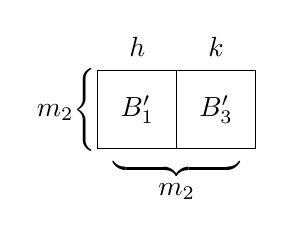
\begin{tikzpicture}{x=1cm,y=1cm}
        \draw(-0.4,1.5) node{${m_2}\Bigg\{$};
        \draw(0.5,2.3) node{$h$};    \draw(1.5,2.3) node{$k$};
        \draw (0,1) rectangle (1,2); \draw(0.5,1.5) node{$B'_1$};
        \draw (1,1) rectangle (2,2); \draw(1.5,1.5) node{$B'_3$};
        \draw(1,.6) node{$\underbrace{\hskip 1.6cm}_{\textstyle  m_2}$};
  \end{tikzpicture}}} ~
  \left[
    \begin{array}{c}
      x'_1 + Cx'_2 + c \\
      x'_3
    \end{array}
    \right]
  = 0
\end{align*}

\noindent
se čtvercovou maticí. Vycházejíce ze způsobu zavedení matice
$B'_3$, snadno se přesvědčíme o tom, že matice (8.27) je navíc
regulární. Jediným řešením soustavy (8.26) je potom jak známo
[37, str.77] nulový vektor, takže je také $x'_3 = 0$ a dokazovaný
vztah (8.22) platí.

Došli jsme tedy k tomuto závěru: k vyrovnání
zprostředkujících pozorování s podmínkami můžeme v případě singularity
druhého druhu užít algoritmu ORTON ve stejné úpravě jako při řešení
singulárních úloh typu CU. Připojení matice $B'_3$ v (8.20) lze totiž
jednoduše realizovat postupným doplňováním ortogonalizované
matice $A$ v (7.8) sloupci se strukturou
%
\begin{align*}
  \tag{8.28}
  \vcenter{\hbox{
      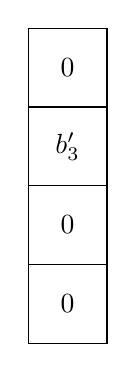
\begin{tikzpicture}[x=1cm,y=1cm]
        \draw (2,3) rectangle (3,4); \draw (2.5,3.5) node{$0$};
        \draw (2,2) rectangle (3,3); \draw (2.5,2.5) node{$b'_3$};
        \draw (2,1) rectangle (3,2); \draw (2.5,1.5) node{$0$};
        \draw (2,0) rectangle (3,1); \draw (2.5,0.5) node{$0$};
  \end{tikzpicture}}}
  \Punc{,}
\end{align*}

\noindent
kde vektory $b'_3$ mohou být vytvářeny generátorem náhodných čísel.
Dokázali jsme, že tak můžeme najít hodnoty neznámých a opravy,
které řeší úlohu (7.5). Neznámé, odpovídající generovaným
sloupcům, budou rovny nule.


Uvedený závěr platí za předpokladu, že podmínkové rovnice
(5.17) a tedy i celá vyrovnávací úloha byly řešitelné. Najdeme
ještě kritérium pro identifikaci úloh, v nichž si podmínkové
rovnice odporují, a které jsou proto neřešitelné. Aplikujeme-li
při řešení těchto úloh algoritmus ORTON doplněný generátorem
sloupců (8.28), budeme řešit jistou náhradní regulární úlohu
(8.20). Dokážeme, že v takovém přínadě dostaneme, na rozdíl od
řešitelných úloh, nenulový vektor $x'_3$ (8.22). Důkaz je nasnadě:
kdyby totiž platilo $x'_3 = 0$, pak by podle (8.20) vektory
$x'_1$ a $x'_2$
%
musely \orig{81} vyhovovat rovnici
%
\begin{align*}
  \tag{8.29}
  0 = B'_1x'_1 + B'_2x'_2 + \ell_2
\end{align*}

\noindent
a muselo by, v rozporu s předpokladem, existovat i řešení
podmínkových rovnic (3.17). Můžeme tedy tvrdit, že zkoumaná úloha
bude řešitelná právě tehdy, bude-li vektor $x'_3$ nulový. Při
užití procedury ORTON3 mohou být složky vektoru $x'_3$ nalezeny
analogicky jako ostatní neznámé. Budou uloženy v posledním sloupci
matice $W$ (7.8) v pozicích, které odpovídají řádkům,
generovaným podle schematu (8.16).
